% Black body radiation curves for Wien's Law
% Wien approximation: f(x) = C * x^{-2} * exp(-a/x), peak at x = a/2
% Non-crossing guaranteed: for a1 < a2, exp(-a1/x) > exp(-a2/x) for all x > 0
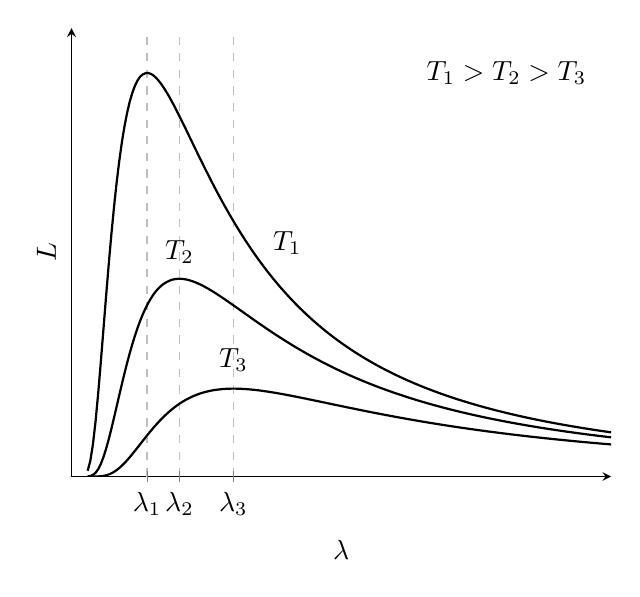
\begin{tikzpicture}
  \begin{axis}[
      xmin=0, xmax=5, ymin=0, ymax=5,
      axis x line=bottom, axis y line=left,
      xlabel=$\lambda$, ylabel=$L$,
      xtick=\empty, ytick=\empty,
      extra x ticks={0.70, 1.00, 1.50},
      extra x tick labels={$\lambda_1$, $\lambda_2$, $\lambda_3$},
      extra x tick style={grid=major, grid style={dashed}},
      samples=200,
    ]
    % T1 (hottest): a=1.4, peak at 0.70
    \addplot[thick, domain=0.15:5] {16.3 * x^(-2) * exp(-1.4/x)};
    % T2: a=2.0, peak at 1.00
    \addplot[thick, domain=0.15:5] {16.3 * x^(-2) * exp(-2.0/x)};
    % T3 (coolest): a=3.0, peak at 1.50
    \addplot[thick, domain=0.15:5] {16.3 * x^(-2) * exp(-3.0/x)};
    % Curve labels (above and right of each curve's descent)
    \node at (axis cs:2.0,2.6) {$T_1$};
    \node at (axis cs:1.0,2.5) {$T_2$};
    \node at (axis cs:1.5,1.3) {$T_3$};
    \node[anchor=west] at (axis cs:3.2,4.5) {$T_1 > T_2 > T_3$};
  \end{axis}
\end{tikzpicture}
